\documentclass[10pt,english]{article}

\usepackage{fourier}

\usepackage[]{graphicx}
\usepackage[]{color}
\usepackage{xcolor}
\usepackage{alltt}
\usepackage{listings}
\usepackage[T1]{fontenc}
\usepackage[utf8]{inputenc}
\setlength{\parskip}{\smallskipamount}
\setlength{\parindent}{5ex}
\usepackage{indentfirst}
\usepackage{listings}
\usepackage{setspace}
\usepackage{hyperref}
\usepackage{url}
\hypersetup{
    colorlinks=true,
    linkcolor=auburn,
    filecolor=magenta,      
    urlcolor=blue, urlsize=2em
}

% Set page margins
\usepackage[top=100pt,bottom=100pt,left=68pt,right=66pt]{geometry}

% Package used for placeholder text
\usepackage{lipsum}

% Prevents LaTeX from filling out a page to the bottom
\raggedbottom


\usepackage{fancyhdr}
\fancyhf{} 
\fancyfoot[C]{\thepage}
\renewcommand{\headrulewidth}{0pt} 
\pagestyle{fancy}

\usepackage{titlesec}
\titleformat{\chapter}
   {\normalfont\LARGE\bfseries}{\thechapter.}{1em}{}
\titlespacing{\chapter}{0pt}{50pt}{2\baselineskip}

\usepackage{float}
\usepackage{verbatim}
\floatstyle{plaintop}
\restylefloat{table}

\usepackage[tableposition=top]{caption}


\definecolor{light-gray}{gray}{0.95}

\renewcommand{\contentsname}{Índice}

\begin{document}


\begin{titlepage}
	\clearpage\thispagestyle{empty}
	\centering
	\vspace{2cm}

	
	{\Large  Teste e Qualidade de Software \par}
	\vspace{0.5cm}
	{\small Professor: \\
	Ilídio Oliveira\par}
	\vspace{4cm}
	{\Huge \textbf{HW1: Qualidade do Ar}} \\
	\vspace{1cm}
	\vspace{4cm}
	{\normalsize Hugo Paiva de Almeida, 93195
	   \par}
	\vspace{2cm}

    
\includegraphics[scale=0.20]{logo_ua.png}
    
    \vspace{2cm}
    
	{\normalsize DETI \\ 
		Universidade de Aveiro \par}
		
	{\normalsize 14-05-2021 \par}
	\vspace{2cm}
		
	
	\pagebreak

\end{titlepage}
\tableofcontents{}
\clearpage

\section{Introdução}

\subsection{Visão Geral do Trabalho}

\par Este trabalho consistiu no desenvolvimento de uma aplicação em \textit{Spring Boot} de modo a fornecer o serviço e respetiva \textit{interface Web}, em \textit{Angular}, com informações atuais sobre a qualidade do ar de uma determinada localização bem como estatísticas da \textit{cache} implementada. O maior foco do trabalho traduziu-se nos testes, com cerca de 70 desenvolvidos, bem como a implementação em \textit{pipelines} de integração contínua de modo a assegurar a execução de todos os testes automaticamente.

\par Para se obter as informações da qualidade do ar, que incluem valores de diversos poluentes do ar, bem como a qualidade geral do ar, foram utilizadas duas \textit{APIs}: a disponibilizada pela empresa \textit{OpenWeather Ltd} e a disponibilizada pelo projeto \textit{The World Air Quality}. Ao realizar um pedido de informações através de coordenadas, o serviço irá primeiramente verificar se existe alguma entrada na \textit{cache} com essas coordenadas e, em caso negativo, irá aceder à última \textit{API}, uma vez que geralmente possui mais dados e, em caso de erro, tentará aceder à primeira. Já no caso do pedido de informações através de localização, o serviço primeiramente acede à primeira \textit{API} através do serviço de resolução de localização disponibilizado e, após receber as coordenadas do local, realiza o pedido normalmente, como descrito anteriormente.

\par Em relação à \textit{cache}, esta foi implementada com base nas coordenadas, servindo estas como chave de acesso, ficando na base de dados de memória, por defeito, durante 120 segundos. Como forma de auxílio na visualização dos dados da \textit{cache}, para além das métricas pedidas, foi também implementado um histórico de pedidos à \textit{API}, cada um com a respetiva referência de acesso ou não à \textit{cache}.

\subsection{Limitações}

\par Uma vez que a \textit{cache} foi preparada para guardar informações relativas a pedidos de informações sobre a qualidade do ar com coordenadas, sempre que um utilizador realiza um pedido para obter informações sobre uma dada localização, é sempre necessário o acesso à \textit{API} externa de resolução para coordenadas, antes do acesso à \textit{cache}. 

\par Apesar de existir vontade para tal, visto que ao implementar todos os testes em \textit{pipelines} de Integração Contínua com configuração de \textit{Selenium} em \textit{Docker} e execução destes testes automaticamente se perdeu bastante tempo, a aplicação cingiu-se à funcionalidade pedida de informações atuais da qualidade do ar, acabando por se explorar pouco as \textit{APIs} em troca de maior foco nos testes.

\clearpage

\section{Especificação do Produto}

\subsection{Espetro funcional e Interações Suportadas}

\par Como utilizador da \textit{interface Web}, é possível aceder às informações atuais da qualidade do ar através de pesquisa por coordenadas e localização. Para além disso, todo o histórico de pedidos e estatísticas referentes à \textit{cache} estão disponíveis, permitindo um maior controlo sobre o funcionamento da mesma.

\par Como utilizador da \textit{REST API}, é possível obter as mesmas informações que um utilizador da \textit{interface Web} mas, de forma mais crua, em \textit{JSON}, permitindo a integração destes dados em outras plataformas.

\subsection{Arquitetura do Sistema}

\par Como mencionado anteriomente, a arquitetura baseia-se em três componentes chave:

\begin{itemize}
    \item Aplicação Web em \textit{Angular}
    \item Serviço em \textit{Spring Boot}
    \item \textit{APIs} Externas
\end{itemize}

\begin{figure}[h]
    \centering
    \includegraphics[width=400]{images/arch.png}
    \caption{Arquitetura do Sistema}
\end{figure}

\par O fluxo deste sistema centra-se no serviço, onde são recebidos os pedidos do cliente, guardados os dados de \textit{cache} e feitos os pedidos às \textit{APIs} externas. Caso o utilizador queira obter informações relativas à qualidade atual do ar, fará um pedido à \textit{REST API} do serviço que, caso necessite de resolver a localização, irá aceder à \textit{API} externa \textit{OpenWeatherMap}, de modo a obter as coordenadas. Tendo as coordenadas, quer seja através da resolução da localização ou através de envio direto do cliente, o serviço verifica se existem informações referentes às mesmas em \textit{cache}, através de uma base de dados em memória \textit{H2}. Caso isto se verifique, estas são retornadas, em caso contrário, são feitos pedidos às \textit{APIs} externas, primeiramente à \textit{AQICN} e, em caso de erro, à \textit{OpenWeatherMap}.

\par Em relação às informações de estatísticas da \textit{cache}, sempre que o serviço recebe um pedido, irá verificar à base de dados as informações guardadas e retornará a lista de pedidos anteriores ou o número de pedidos, acessos à \textit{cache} e falhas de acessos à \textit{cache}.

\par Para visualizar melhor o serviço, é possível observar o seu diagrama \textit{UML} \href{https://github.com/hugofpaiva/tqs-p1/tree/main/report/source/images/air-quality-service-uml.png}{aqui}.

\subsection{\textit{API} de Documentação}

\par Um desenvolvedor pode obter informações relativas à qualidade do ar através de coordenadas ou localização, bem como aceder a informações referentes ao funcionamento da \textit{cache}. 

\par De modo a documentar os \textit{endpoints} da \textit{API}, recorreu-se à ferramenta \textit{Swagger}, ficando esta disponível no \textit{endpoint} \textit{/api/swagger-ui/index.html}:

\begin{figure}[h]
    \centering
    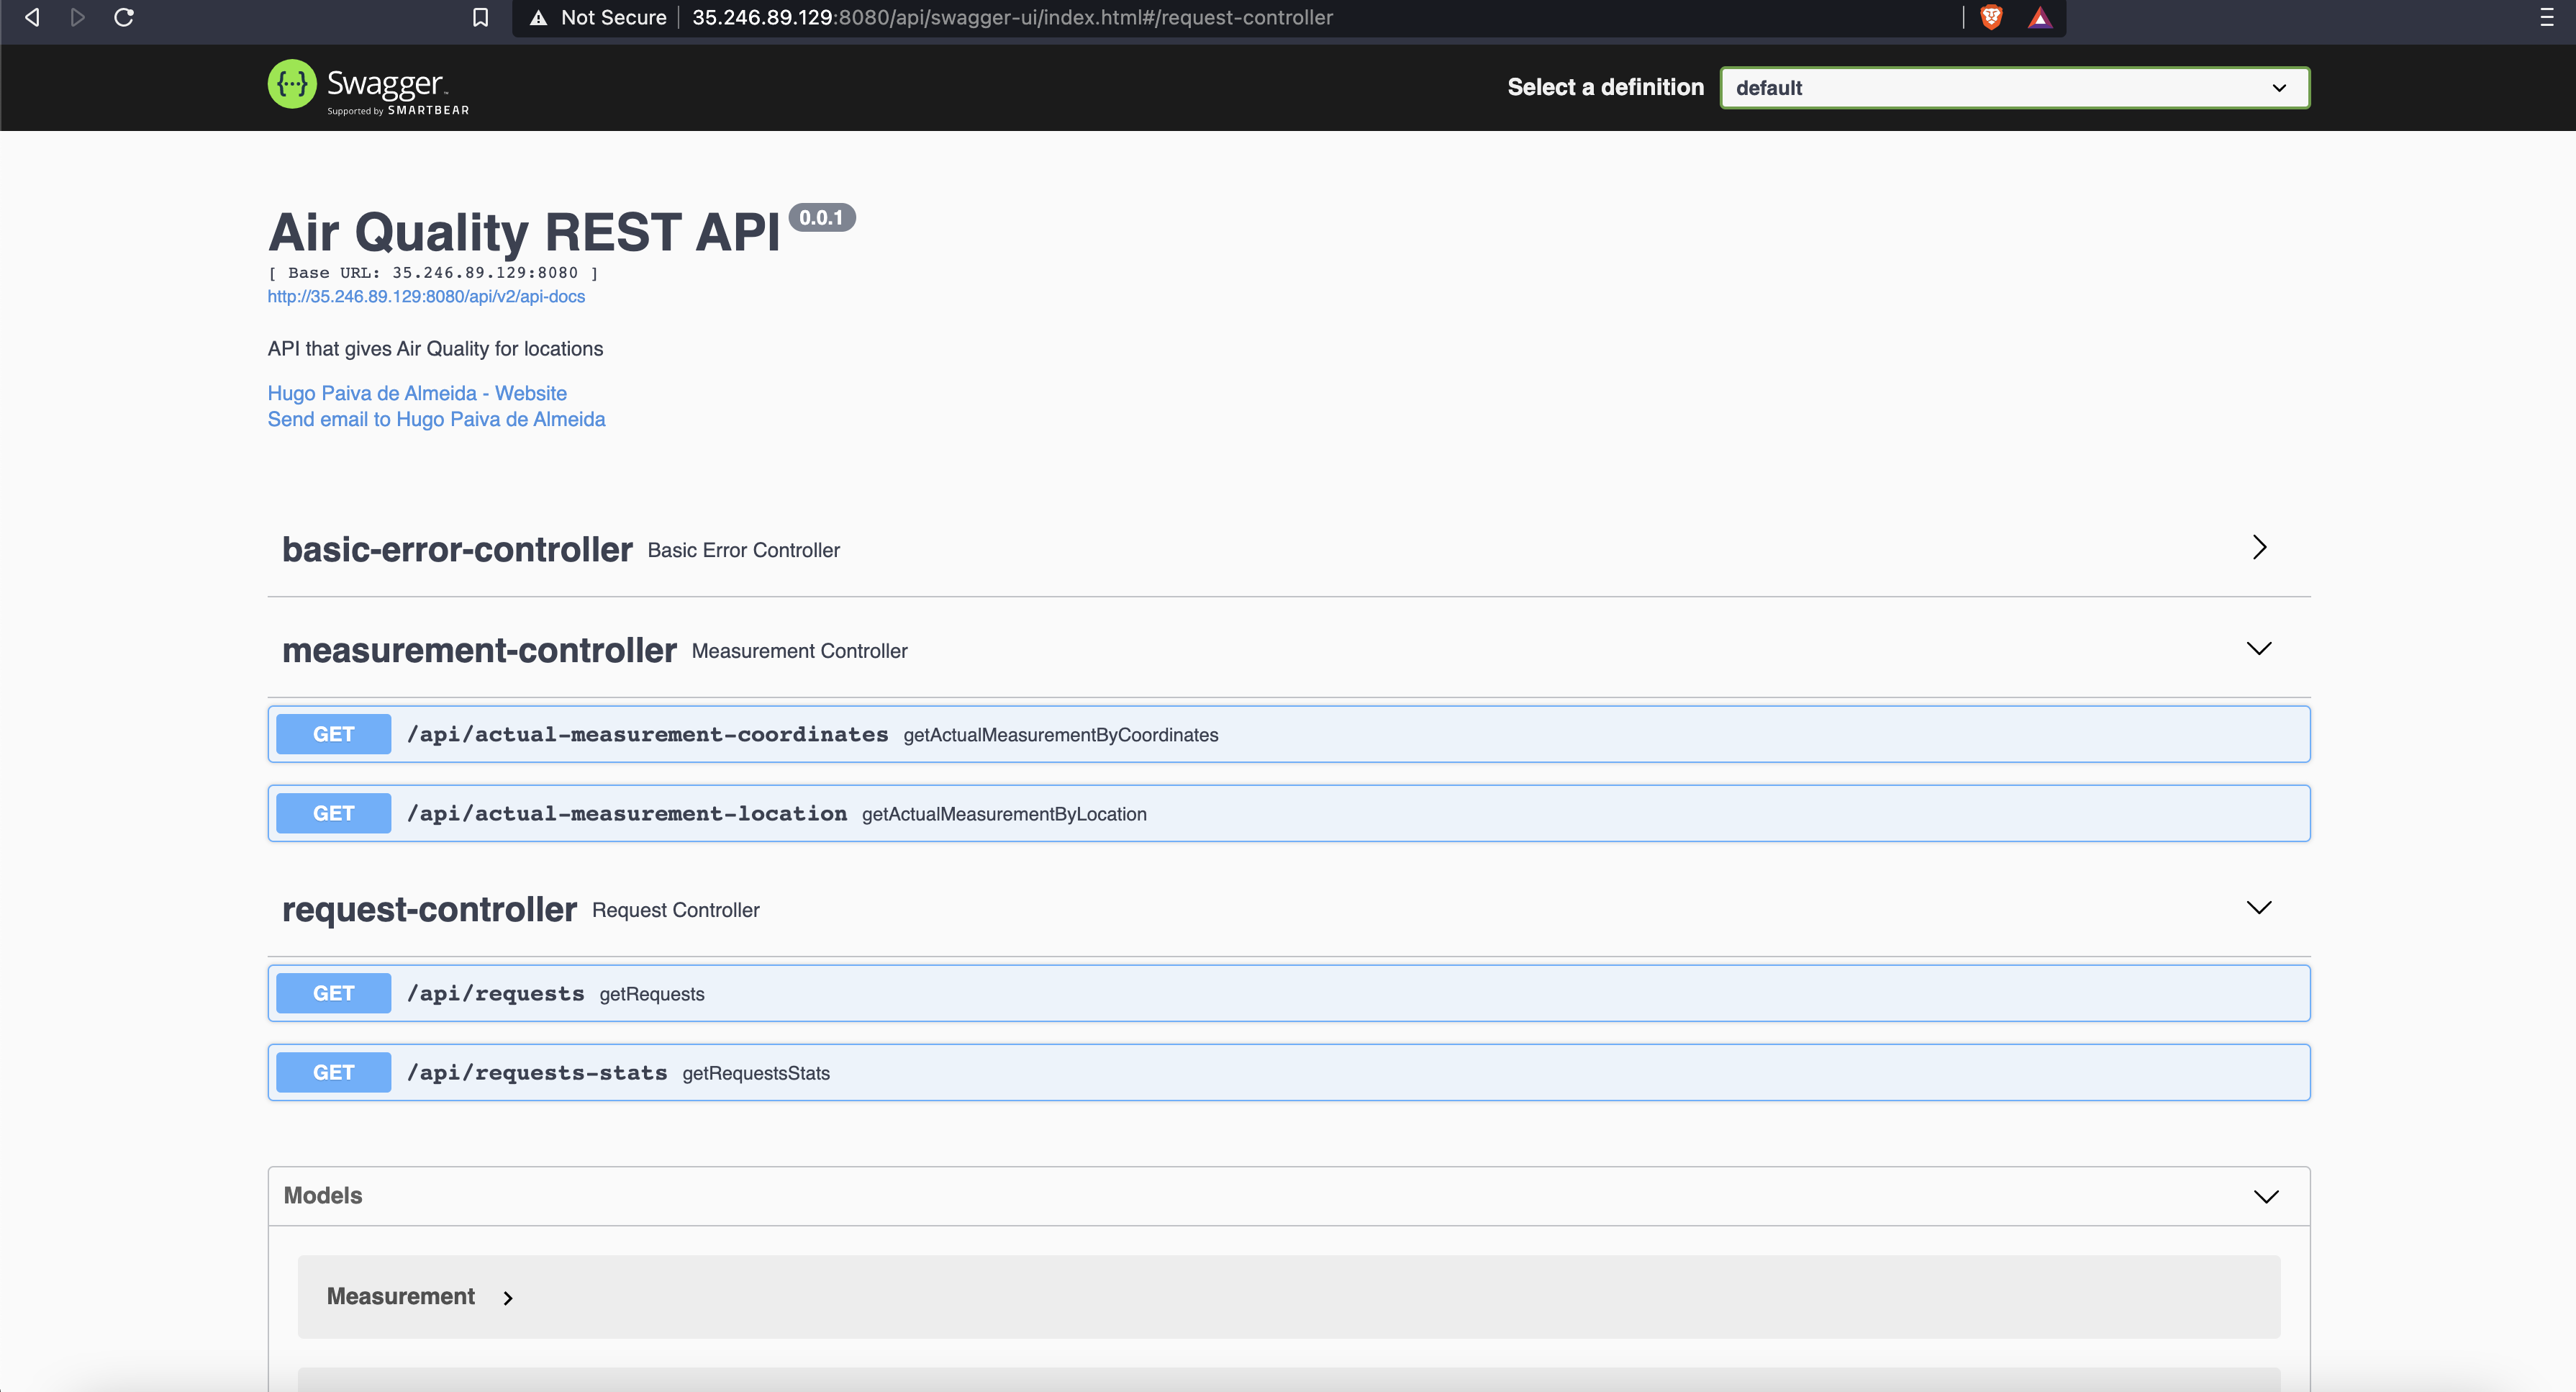
\includegraphics[width=400]{images/swagger.png}
    \caption{Documentação da \textit{REST API} através do \textit{Swagger}}
\end{figure}

\section{Garantia de Qualidade}

\subsection{Estratégia de testes}

\par Tentou-se seguir uma aproximação \textit{Test-Driven Development (TDD)} sempre que possível, no entanto nem sempre se conseguiu fazer os testes antes de uma versão funcional da componente em que se estava a trabalhar. Apesar disto, reconhece-se que esta abordagem é excelente para se perceber logo desde o início todos os cenários que uma determinada componente irá ter de enfrentar.

\clearpage 

\subsection{Testes Unitários e de Integração}

\par Foram feitos testes unitário para todas as classes referentes à funcionalidade do serviço, com objetos \textit{Mock}, sempre que possível. Para definir os testes, pensou-se em todos os cenários possíveis de falha do funcionamento da classe, assegurando que existiria o levantamento de exceções nestes casos, e nos casos normais de uso. Tentou-se sempre descrever o objetivo dos testes através do título da função de teste.

\par Um bom exemplo destes testes são os testes da \textit{Cache} e dos \textit{Services}, onde em ambos se utilizam vários objetos \textit{Mock} que são injetados na instância da classe que se vai testar:

\begin{figure}[h]
    \centering
    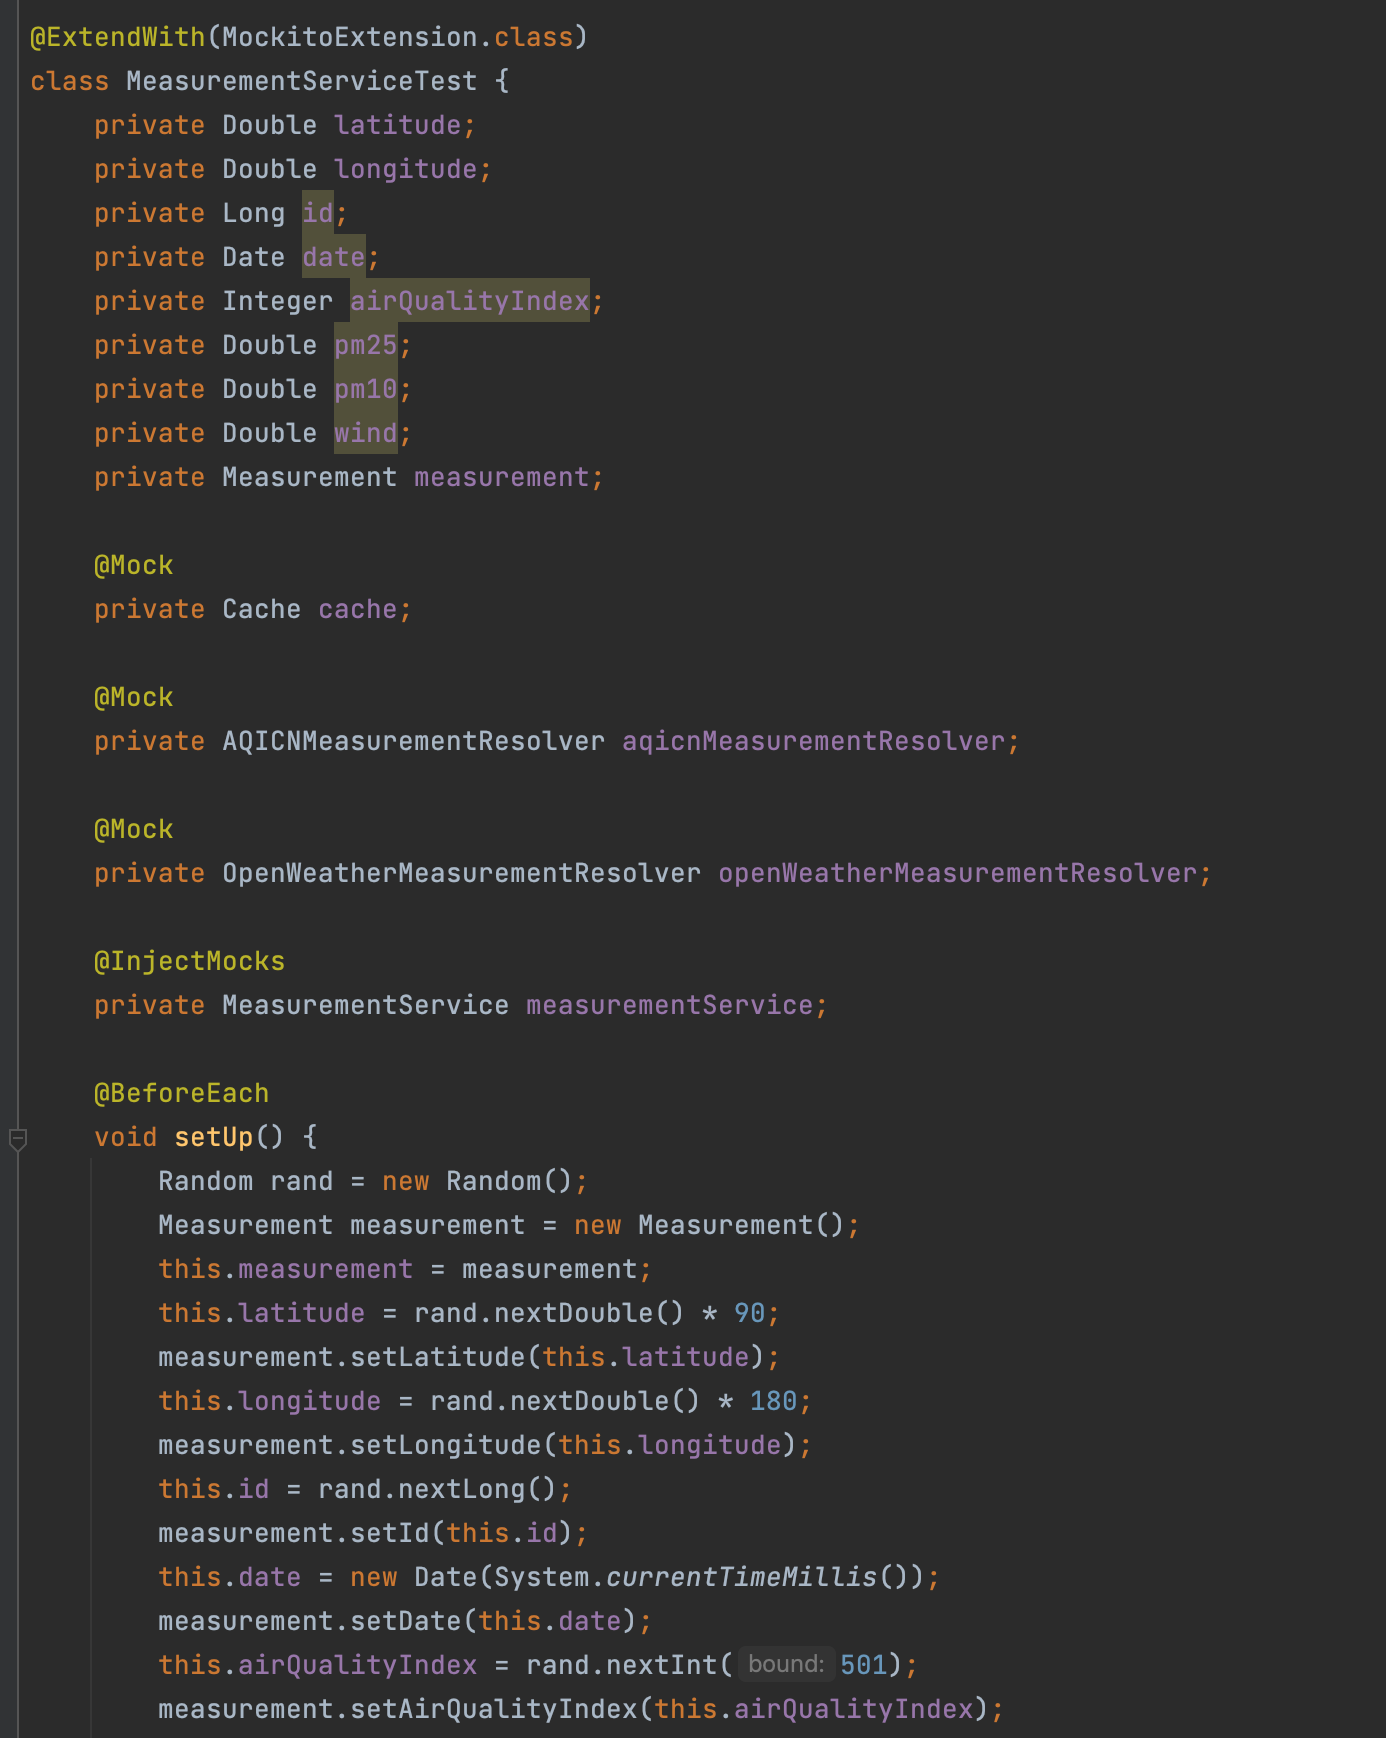
\includegraphics[width=300]{images/measurements-services-tests.png}
    \caption{Classe de testes referente à classe \textit{MeasurementServices} com a exitência de vários \textit{Mocks}}
\end{figure}

\clearpage

\par Em relação aos testes de integração, foram feitos testes por cada componente \textit{Controller}, de modo a testar:

\begin{itemize}
    \item Comportamento do \textit{Controller} sem a utilização de uma \textit{HTTP-REST framework} com os testes \textit{MeasurementControllerMockMvcMockServiceTest} e \textit{RequestControllerMockMvcMockServiceTest}, utilizando como objeto \textit{Mock} a classe dos \textit{Services} de cada um
    
    \item Comportamento do \textit{Controller} com a \textit{REST API} a funcionar do lado do servidor e todos componentes a participar com os testes \textit{MeasurementControllerMockMvcIT} e \textit{RequestControllerMockMvcIT}
    
    \item Comportamento do \textit{Controller} com a \textit{REST API} a funcionar do lado do servidor, todos os componentes a participar e um cliente \textit{HTTP} envolvido com os testes \textit{MeasurementControllerTemplateIT} e \textit{RequestControllerTemplateIT}
\end{itemize}

\begin{figure}[h]
    \centering
    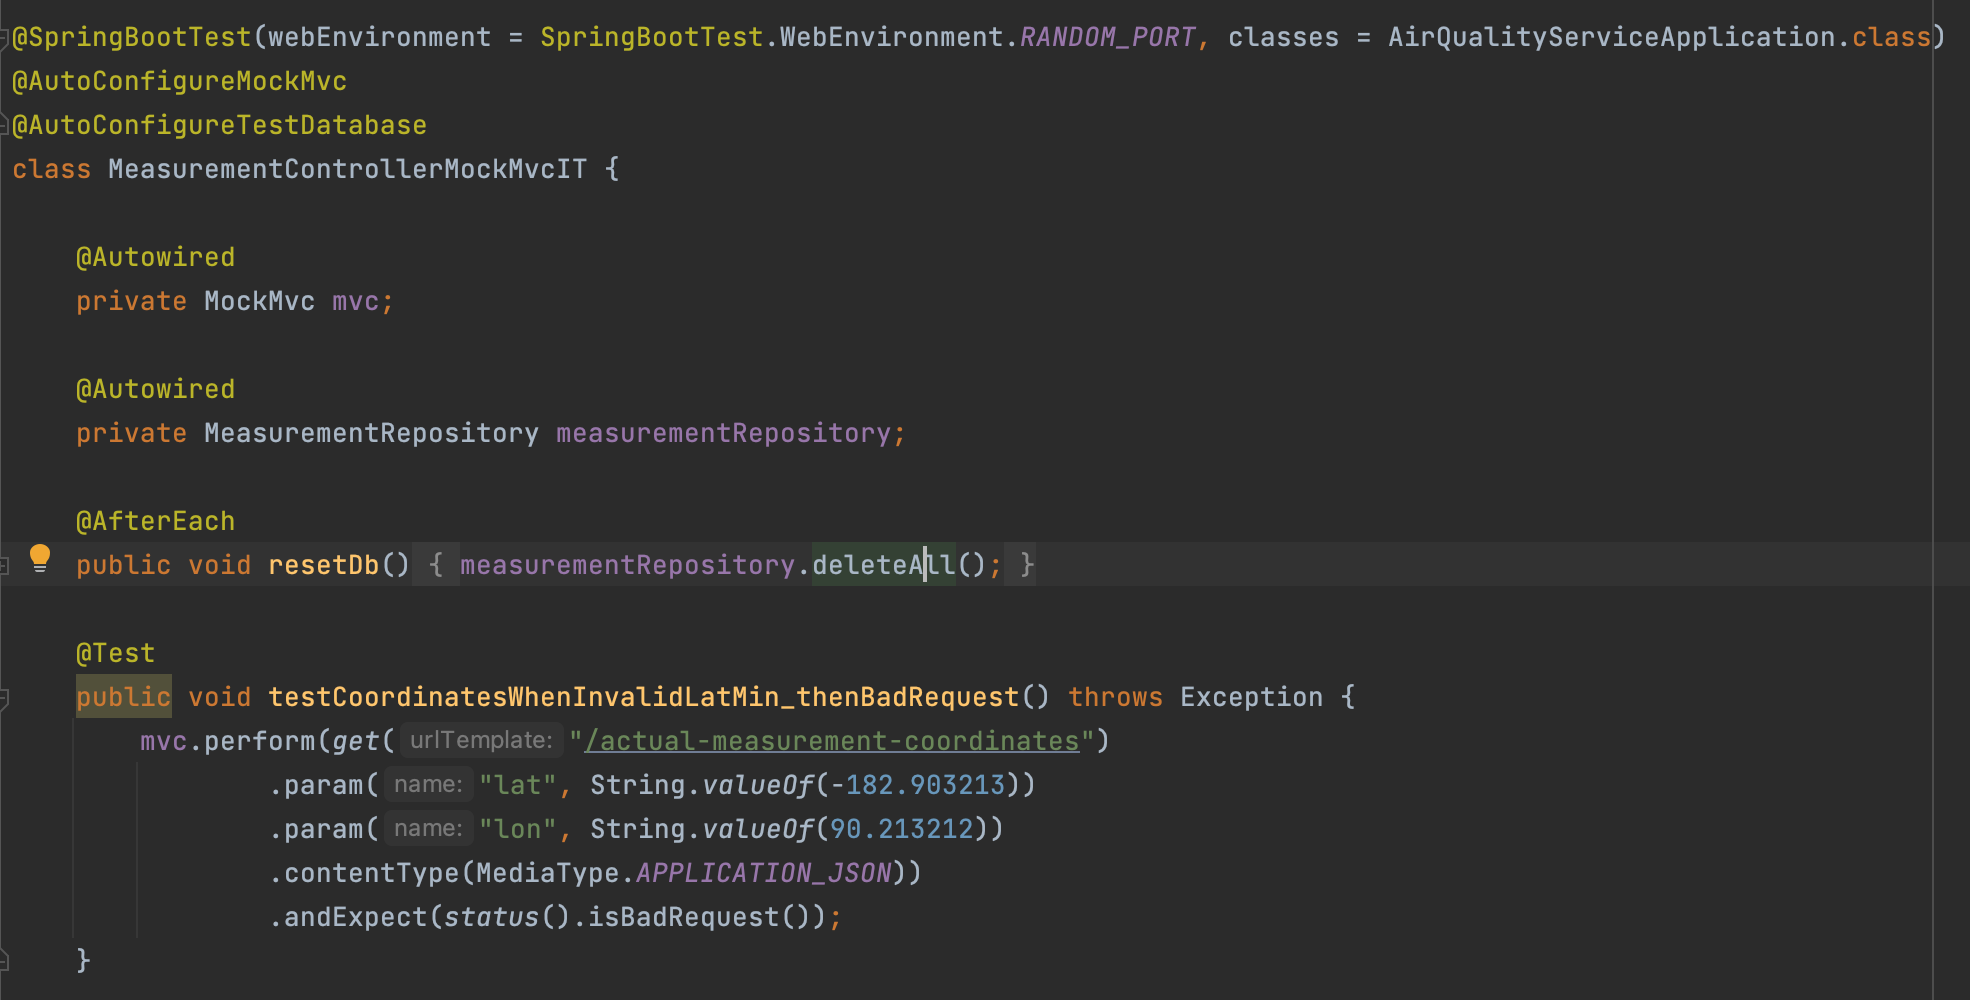
\includegraphics[width=400]{images/measurements-template-tests.png}
    \caption{Exemplo de teste do \textit{MeasurementController} com a \textit{REST API} a funcionar do lado do servidor e um cliente \textit{HTTP} envolvido}
\end{figure}

\clearpage

\subsection{Testes Funcionais}

\par Uma vez que se queria envolver os testes funcionais no processo automático de testes com Integração Contínua, perdeu-se bastante tempo de modo a configurar o \textit{Selenium} para utilizar um \textit{DockerBrowser}. Nestes testes, além de se testar casos normais de uso que um cliente teria, também se assegurou que a aplicação \textit{Web} responderia com mensagens de erro indicativas do tipo de problema encontrado.

\par O endereço utilizado para fazer os pedidos é o \textit{172.17.0.1} uma vez que, estando o \textit{browser} a correr num \textit{container Docker}, para este aceder à \textit{API} que está a ser executada explicitamente para estes testes de acordo com a anotação \textit{@SpringBootTest(webEnvironment = SpringBootTest.WebEnvironment.DEFINED\_PORT)}, o mesmo tem de aceder ao \textit{localhost} da máquina que lançou o \textit{container}, o que apenas é possível com aquele endereço em sistemas \textit{Linux}. Também foi necessária uma configuração especial a nível de endereço para onde vão os pedidos à \textit{API} no \textit{Angular}, de modo a que estes testes corram sem problemas.

\begin{figure}[h]
    \centering
    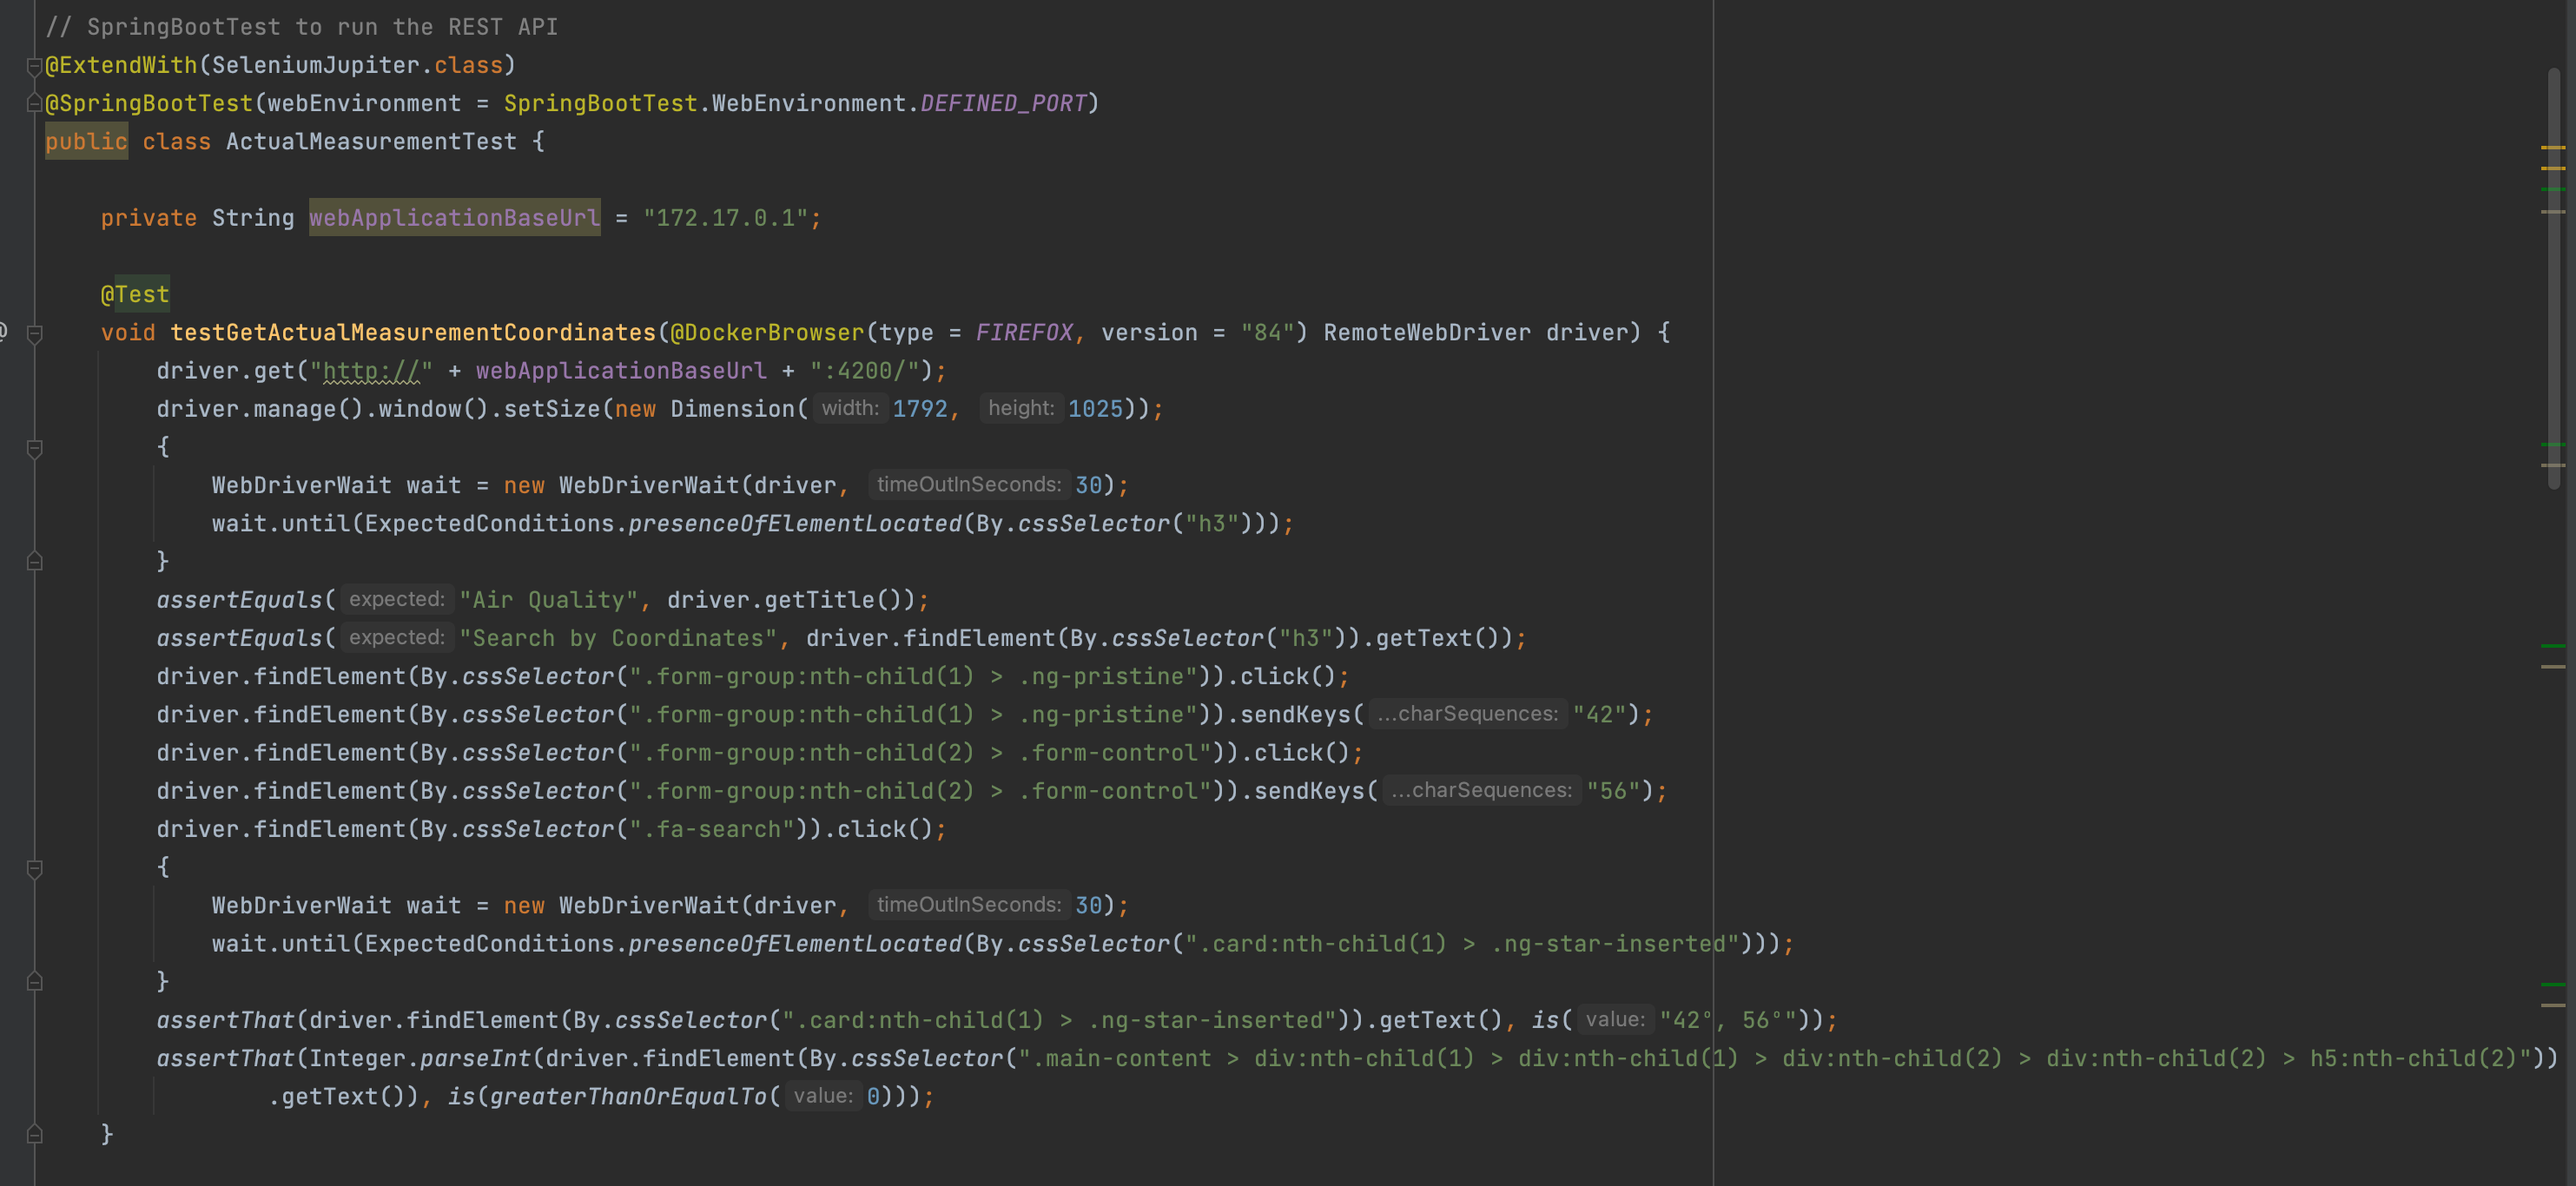
\includegraphics[width=450]{images/selenium-test.png}
    \caption{Exemplo de testes do \textit{Selenium} com \textit{DockerBrowser}}
\end{figure}

\clearpage

\subsection{Análise de Código Estático}

\par Para a análise de código estático, foi criado um servidor próprio do \textit{SonarQube} na \textit{Google Cloud}. Este servidor encontra-se no endereço \href{http://34.89.73.181:9000}{http://34.89.73.181:9000} com as seguintes credenciais:

\begin{itemize}
    \item \textbf{Login:} admin
    \item \textbf{Password:} tqs-p1
\end{itemize}

\begin{figure}[h]
    \centering
    
\includegraphics[width=450]{images/instancia-sonar-google.png}
    \caption{\textit{VM} com uma instância do \textit{SonarQube}}
\end{figure}

\begin{figure}[h]
    \centering
    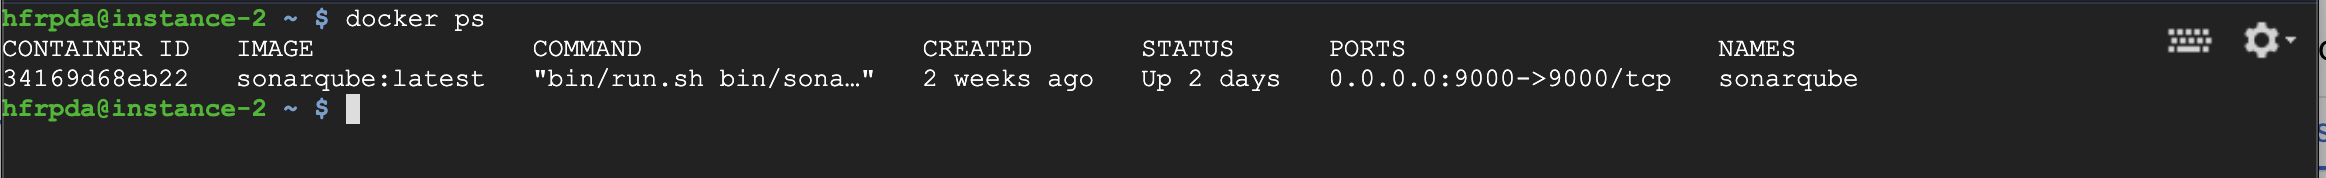
\includegraphics[width=450]{images/docker-ps-sonar.png}
    \caption{\textit{SonarQube} em um \textit{container Docker}}
\end{figure}

\par Através desta ferramenta foi possível ir verificando a qualidade do código bem como, por meio da Integração Contínua, se o novo código adicionado seguia os requisitos mínimos de qualidade de código, sendo que foram utilizados os que existem por defeito:

\begin{figure}[h]
    \centering
    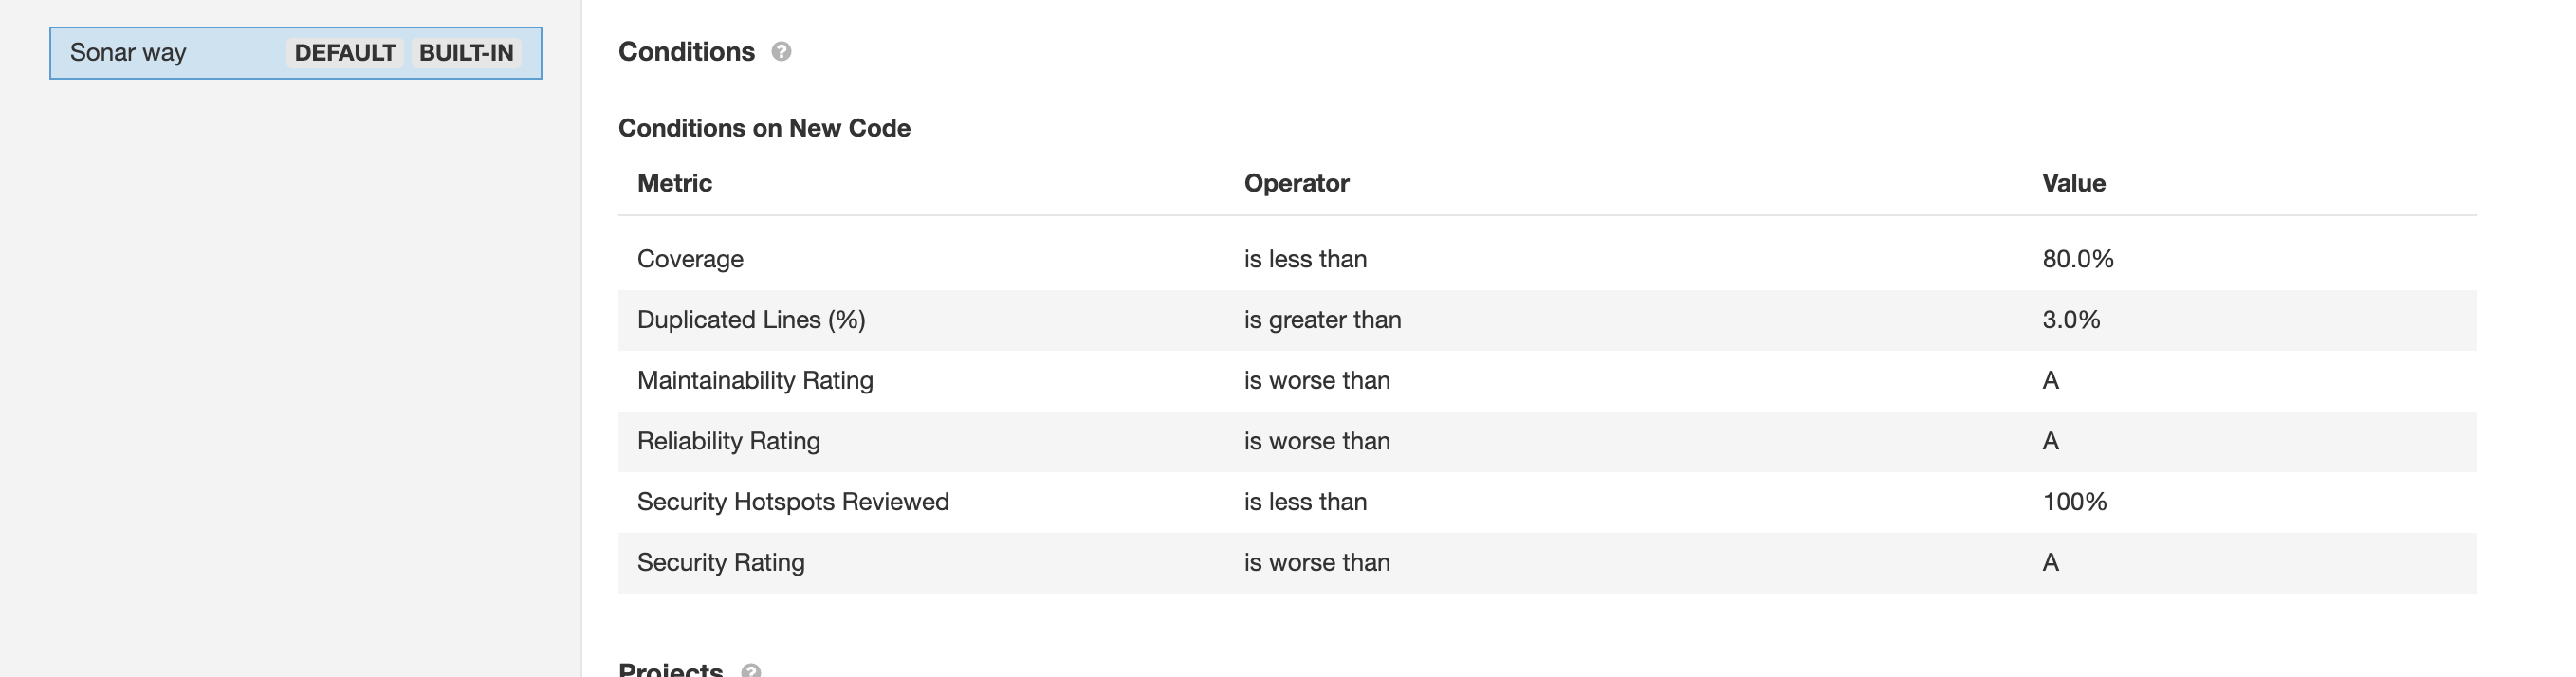
\includegraphics[width=400]{images/quality-gate.png}
    \caption{Requisitos mínimos de qualidade de código definidos no \textit{SonarQube}}
\end{figure}

\clearpage


\par Ao longo do desenvolvimento foram detetados alguns \textit{Code Smells} mais graves que rapidamente foram resolvidos, comprovando a utilidade desta ferramenta. O resultado final, após a execução de todos os testes e resolução dos \textit{Code Smells} mais graves é o seguinte:

\begin{figure}[h]
    \centering
    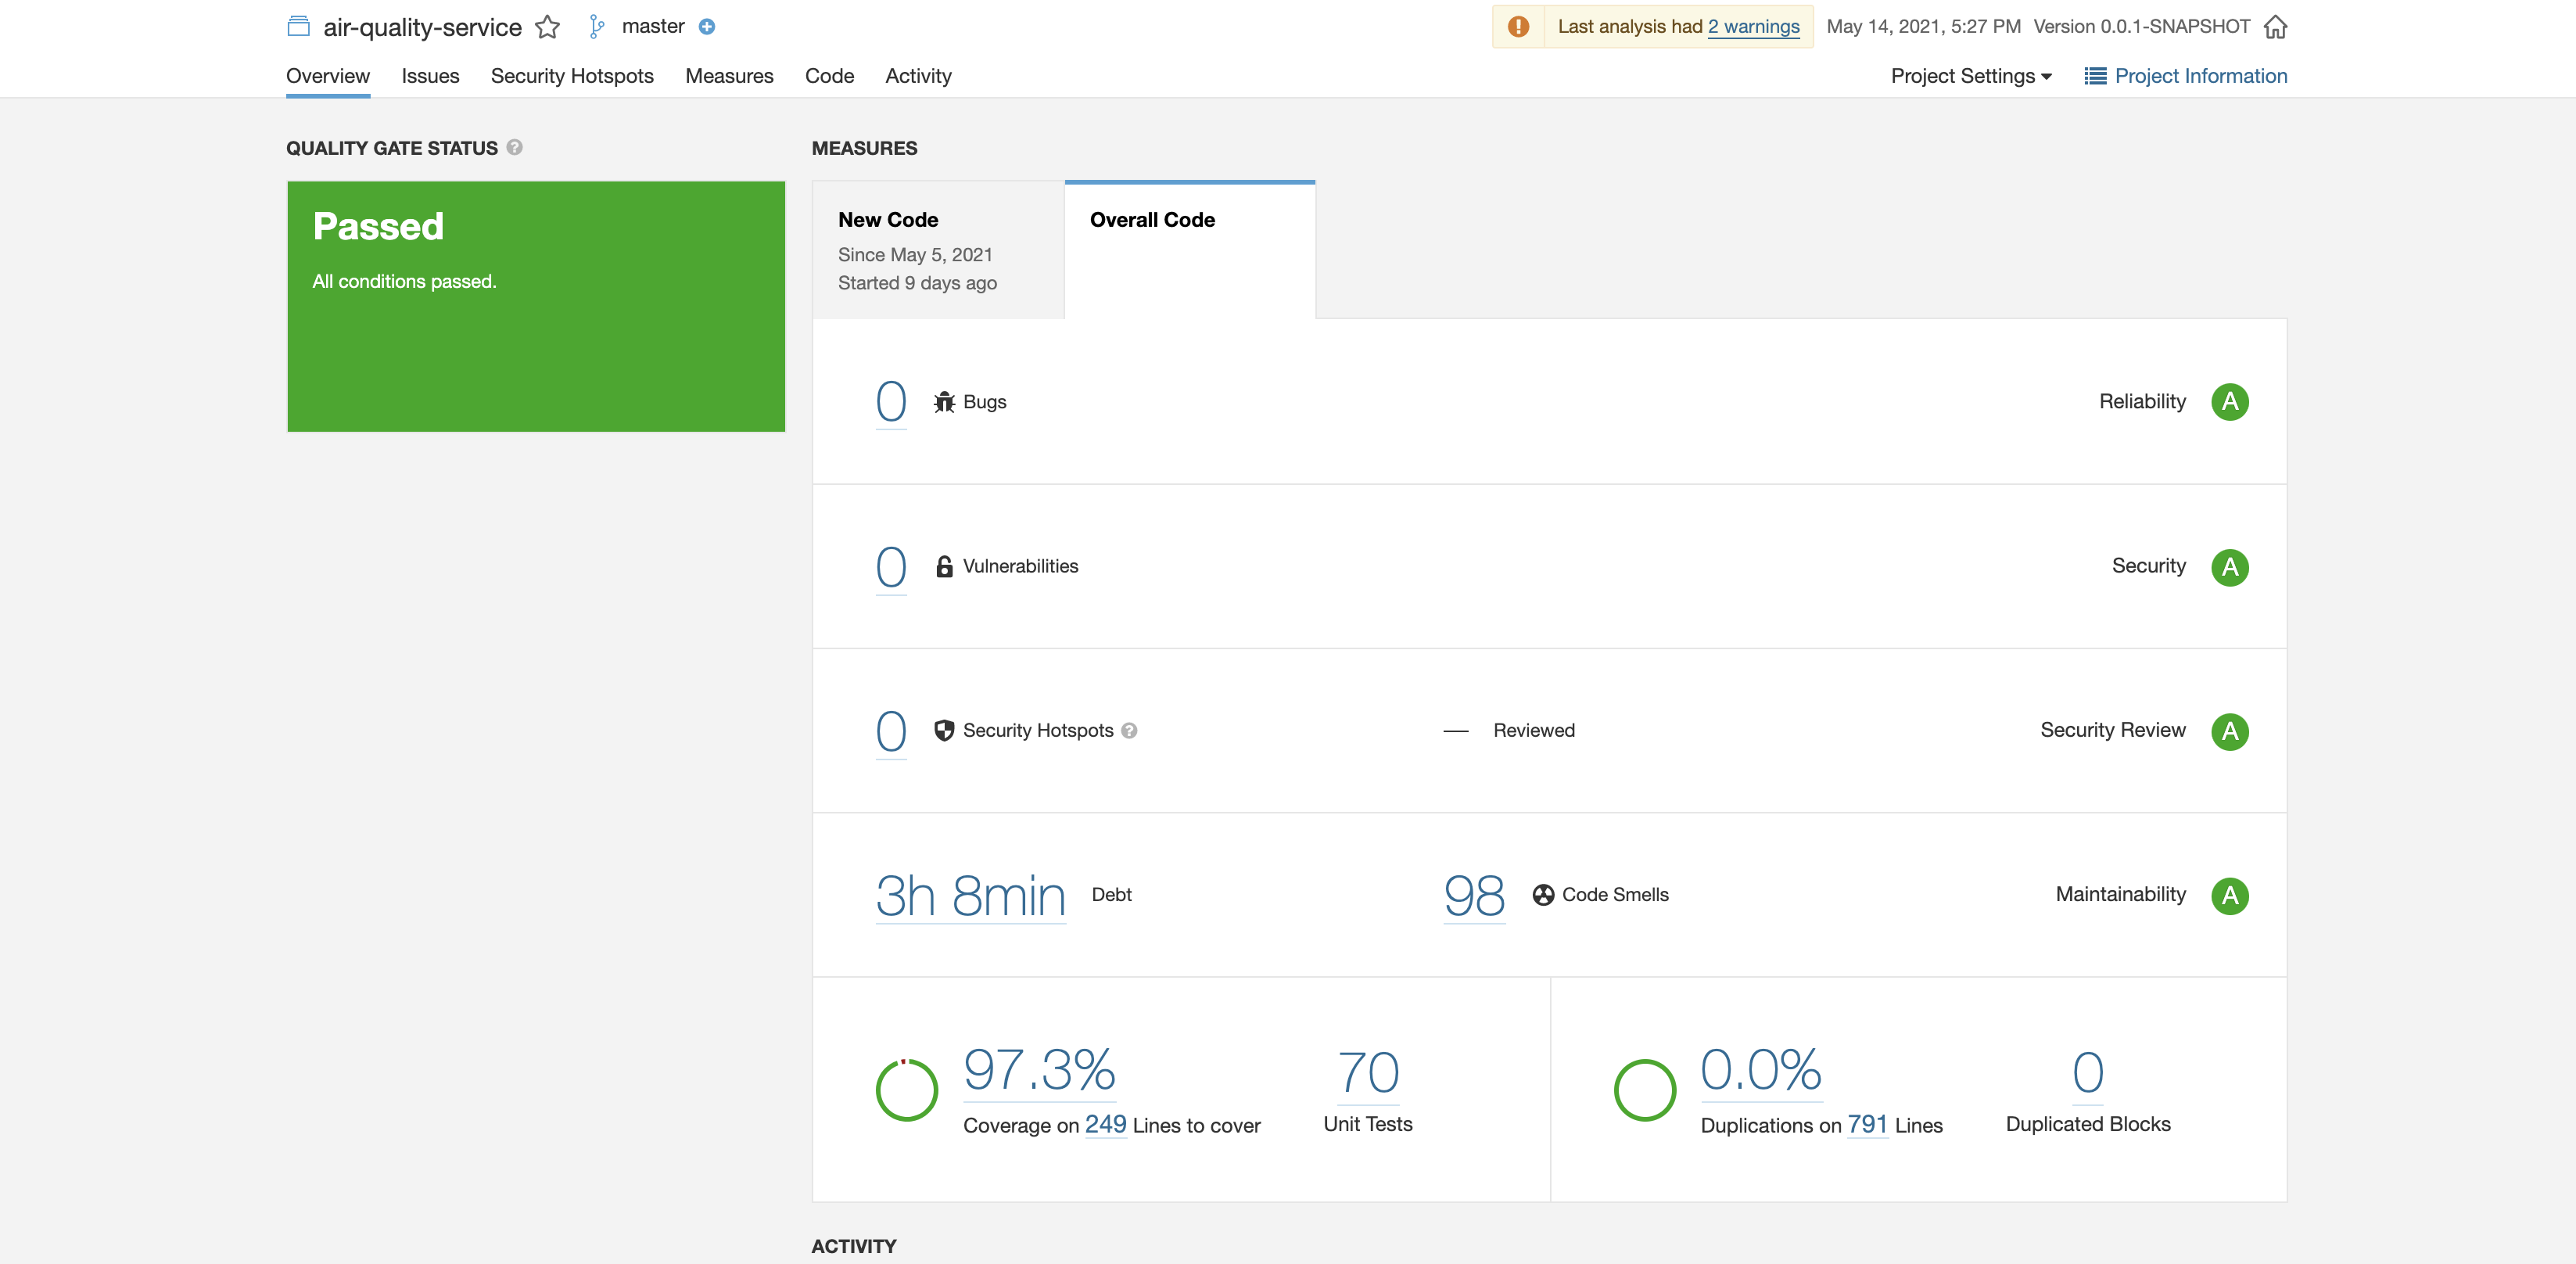
\includegraphics[width=425]{images/sonar-qube-overview.png}
    \caption{\textit{SonarQube Overview}}
\end{figure}

\par Em suma, excedeu-se por muito os requisitos mínimos, tendo um \textit{Code Coverage} de praticamente de 100\%, o que revela a eficácia dos testes produzidos.

\clearpage

\subsection{\textit{Pipeline} de Integração Contínua}

\par Em relação à \textit{Pipeline} de Integração Contínua foram definidas duas \textit{Pipelines}, uma para testar a \textit{build} do \textit{Angular} e outra para testar o código do \textit{Spring Boot}, enviar o código para análise no \textit{SonarQube} e aprovação segundo os requisitos mínimos. No fundo, sempre que se fazia \textit{push} para a \textit{branch} \textit{main} ou se criava um \textit{pull request} com destino nessa branch, estes testes eram executados, sendo que a \textit{pull request} só era aceite quando no último \textit{commit} os testes fossem executados com sucesso.

\begin{figure}[h]
    \centering
    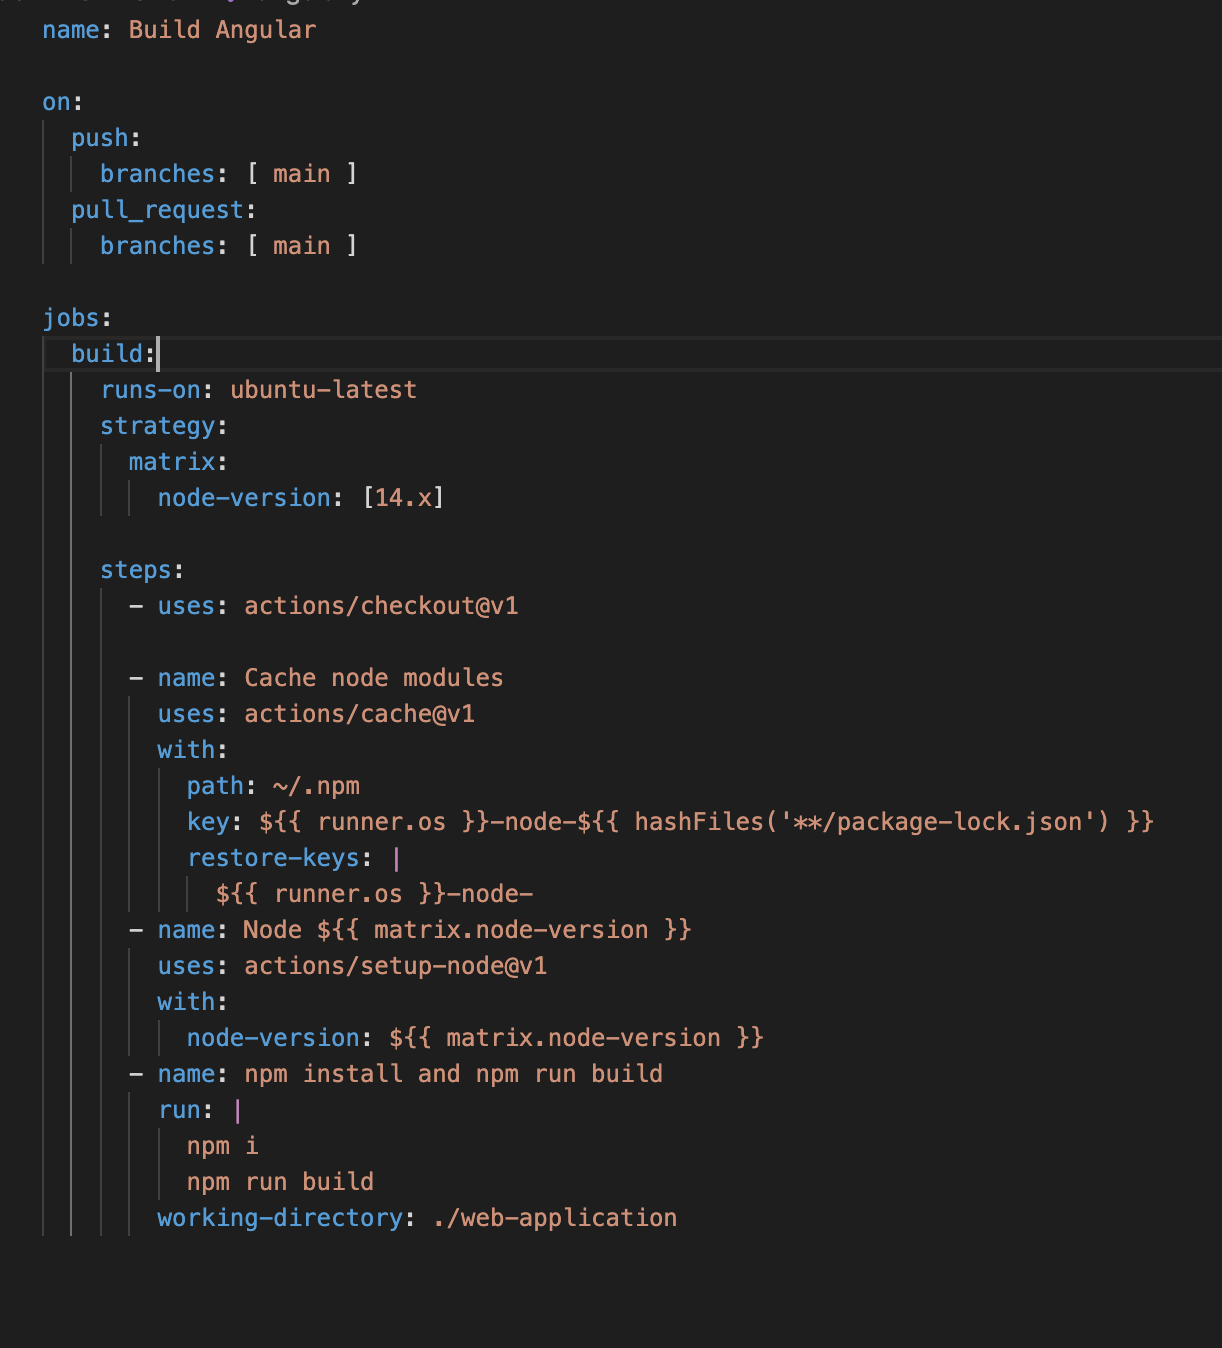
\includegraphics[width=350]{images/pipeline-build-angular.png}
    \caption{\textit{Pipeline Build Angular}}
\end{figure}

\clearpage

\begin{figure}[h]
    \centering
    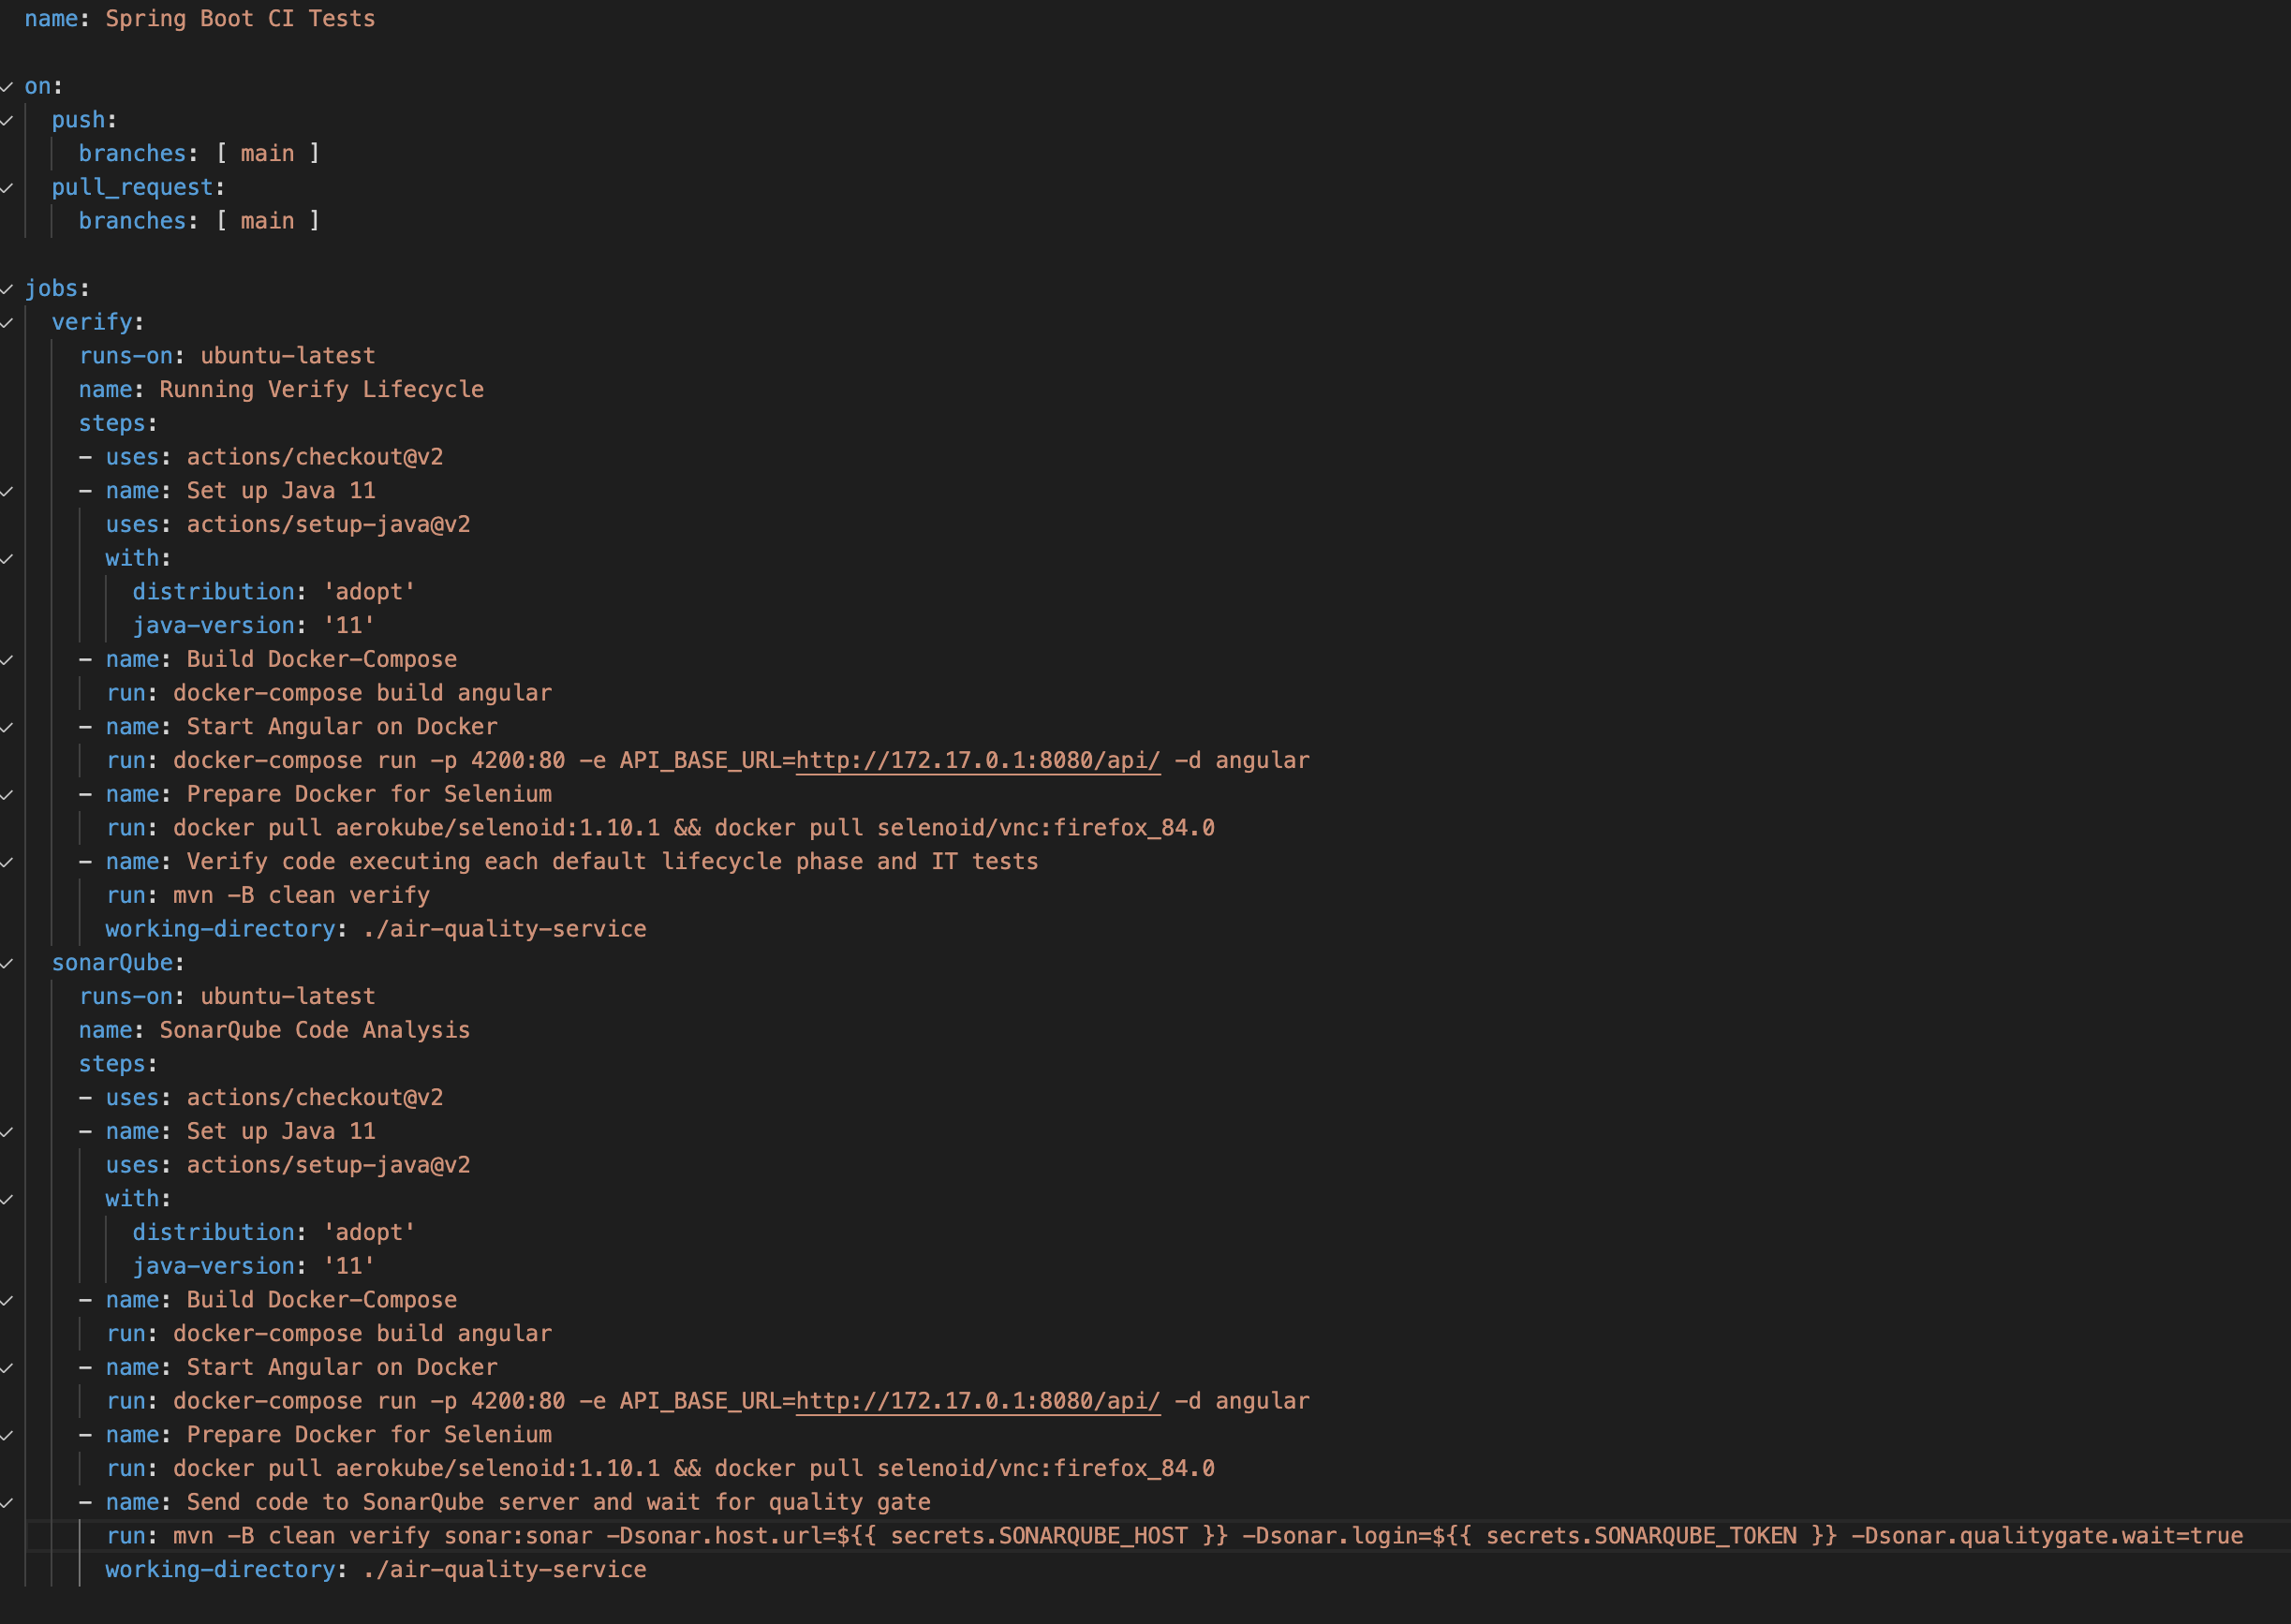
\includegraphics[width=450]{images/pipeline-spring.png}
    \caption{\textit{Pipeline} testes \textit{Spring Boot}}
\end{figure}

\par De notar que, na reta final do trabalho, para permitir a execução dos testes funcionais, a \textit{build} e execução da aplicação \textit{web} em \textit{Angular} em \textit{container Docker} também teve de ocorrer na \textit{pipeline} dos testes do \textit{Spring Boot}.

\clearpage

\section{Conclusão}

\par Para terminar, pensa-se que, de acordo com as metas estabelecidas pelo docente, o trabalho foi bem sucedido. Foi possível desenvolver uma aplicação \textit{Web} e testá-la intensivamente quer manualmente, quer automaticamente através de uma \textit{Pipeline} de Integração Contínua. A eficácia dos testes construídos foi demonstrada, com o auxílio do \textit{SonarQube}, que também alertou para situações relevantes através dos \textit{Code Smells}.

\par Considera-se que os conhecimentos para a realização de testes, bem como de outras ferramentas como \textit{Docker}, \textit{Spring Boot} e \textit{Angular}, foram aprofundados para além da percepção da importância dos testes uma vez que em alguns casos na implementação faltava código para lidar com situações. Segui-se a metáfora do teste de pirâmide, começando pelo desenvolvimento dos testes unitários, seguindo-se os de integração e por fim os funcionais.

\par Este trabalho focou-se principalmente na componente da realização de testes.

\section{Resources}

\par \textbf{Demo:} \url{https://www.youtube.com/watch?v=4_sAMCed5b4}

\par \textbf{Aplicação Web:} \url{http://35.246.89.129/}

\par \textbf{REST API:} \url{http://35.246.89.129:8080/}

\par \textbf{Documentação REST API:} \url{http://35.246.89.129:8080/api/swagger-ui/index.html}

\par \textbf{Repositório:} \href{https://github.com/hugofpaiva/tqs-p1}{https://github.com/hugofpaiva/tqs-p1}

\par \textbf{SonarQube:} \href{http://34.89.73.181:9000}{http://34.89.73.181:9000} com as seguintes credenciais:

\begin{itemize}
    \item \textbf{Login:} admin
    \item \textbf{Password:} tqs-p1
\end{itemize}


\section{Referências}

\bibliographystyle{plain}

\bibliography{biblist}

[1] Material de apoio do Docente

[2] T. W. A. Q. I. project, “API - Air Quality Programmatic APIs” aqicn.org. \url{https://aqicn.org/api/}

[3] “Air Pollution - OpenWeatherMap,” openweathermap.org. \url{https://openweathermap.org/api/air-pollution}

[4] “Automate Your Development Workflow With Github Actions - DZone DevOps,” dzone.com. \url{https://dzone.com/articles/automate-your-development-workflow-with-github-act-1}

[5] “Dockerize a Spring Boot app in 3 minutes,” Docker cloud hosting. Cheap, simple and fast to deploy and manage. \url{https://dockerize.io/guides/docker-spring-boot-guide}

[6] “Try Out SonarQube | SonarQube Docs,” docs.sonarqube.org. \url{https://docs.sonarqube.org/latest/setup/get-started-2-minutes/}

\end{document}

